\section{Arkitektur-overvejelser}\label{sec:arkitektur}
For at skabe et overblik over hvordan informationer skal håndteres i systemet,
og hvordan de forskellige klasser skal kommunikere, har gruppen valgt at lave en domænemodel.
Domænemodellen sikrer at gruppen har en fælles forståelse for systemets opbygning,
og giver en smule klarhed over arkitekturen af systemet.\\

Domænemodellen kan ses på figur (\ref{fig:domain})

\begin{figure}[h]
    \centering
    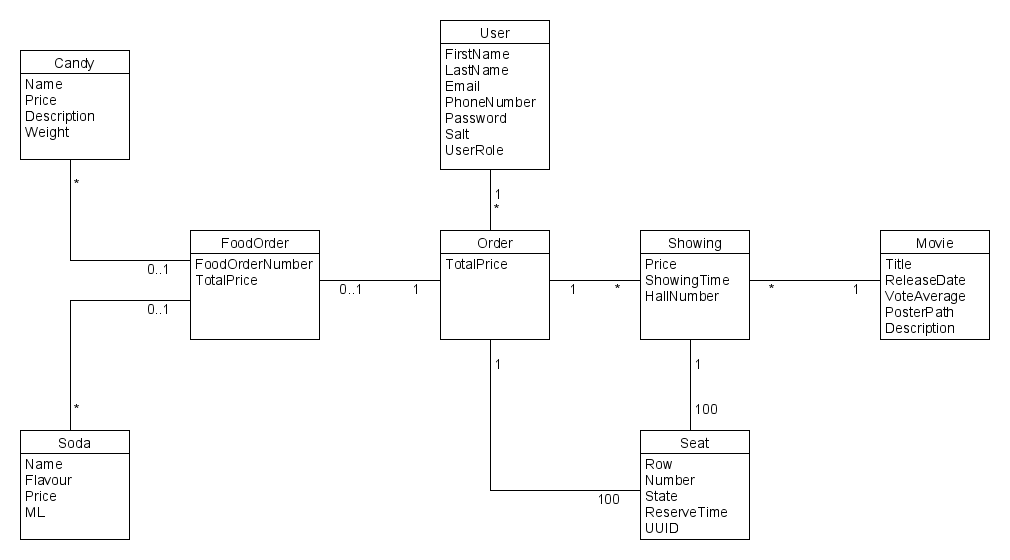
\includegraphics[width=1\textwidth]{figures/Domainmodel.png}
    \caption{Domainmodel}
    \label{fig:domain}
\end{figure}

Domænemodellen er udarbejdet over flere iterationer, og er derfor blevet ændret en del gange.
Venstre side af modellen er ikke blevet implementeret (fra FoodOrder), da gruppen har valgt at fokusere på
en anden user story, nemlig "Create Booking", som resten af domænemodellen beskriver. Dette skyldes at "Create Booking"
giver den største forretningsværdi. \\

Gruppen har på 2. semester arbejdet med trelags arkitektur, og brugt det i det daværende projekt.
Herfor har det givet god mening at bygge det nuværende systemet op efter nogle af de samme principper.
Eftersom undervisningen er blevet mere kompleks, og gruppens evner er blevet udvidet, er systemet endt op med en
N-Tier arkitektur.\\

